
% Created by Chris Schommer-Pries on 2018-01-17.
\documentclass{article}



%%%%%% Tikz  %%%%%%%%%%%%%
\usepackage{tikz}
\usepgflibrary{arrows.meta}

\title{Sandbox}
\author{Everyone}

\begin{document}

\maketitle

\begin{abstract}
    This is a sandbox file, which just means a file where anyone can
    play in the sand. That is anyone can play around with bits of tex
    code before adding them to the main tex file. Hi, this is
    Hari. This is Daniel.
\end{abstract}

\section{Introduction}

Who needs and introduction anyway?

I made this edit concurrent with ``Who needs\ldots''

\subsection{Testing}

Subsections

Building sandcastles in the sandbox.



\section{Commutative diagrams}
Here is a sample commutative diagram in Tikz. 
\begin{center}
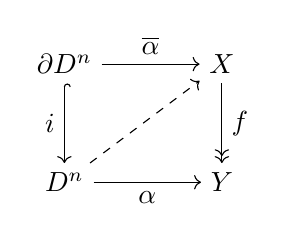
\begin{tikzpicture}
		\node (LT) at (0, 1.5) {$ \partial D^n $};
		\node (LB) at (0, 0) {$ D^n $};
		\node (RT) at (2, 1.5) {$ X $};
		\node (RB) at (2, 0) {$ Y $};
		\draw [{Hooks[right]}->] (LT) -- node [left] {$ i $} (LB);
		\draw [->] (LT) -- node [above] {$ \overline{\alpha} $} (RT);
		\draw [->>] (RT) -- node [right] {$ f $} (RB);
		\draw [->] (LB) -- node [below] {$ \alpha $} (RB);
		
		\draw [->, dashed] (LB) -- node [above left] {$  $} (RT);
		% for adding pullback/pushout symbols
		%\node at (0.5, 1) {$\ulcorner$};  
		%\node at (1.5, 0.5) {$\lrcorner$};
\end{tikzpicture}
\end{center}


\end{document}
